%\documentclass[convert={density=600,outext=.png}]{standalone}
\documentclass[]{standalone}
\usepackage{luatex85}
\usepackage{booktabs}
\usepackage[]{siunitx}
\usepackage{xcolor}
\usepackage{graphicx}
\usepackage{tikz}
\sisetup{range-phrase=--}
\usetikzlibrary{calc}

%\usetikzlibrary{arrows,arrows.meta,positioning,fit,shapes,calc,intersections,matrix, backgrounds}

\begin{document}
	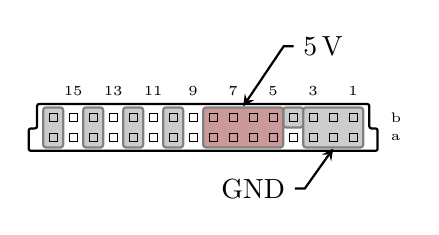
\begin{tikzpicture}[x=2.54mm, y=2.54mm,
		pin/.style = {
			draw,
			rectangle,minimum size=1mm,
			inner sep=0pt},
		arrow/.style = {
			thick,
			->,
			>=stealth,
		},
		]
		% Outline
		\draw[rounded corners=0.75, thick, draw=black, fill=white] (-3.1mm,-1.7mm) -- ++(0mm,2.85mm) -- ++(1.05mm,0mm) -- ++(0mm,3.1mm) -- ++(42.2mm,0mm) -- ++(0mm,-3.1mm) -- ++(1.05mm,0mm) -- ++(0mm,-2.85mm) -- cycle;
		% Marker
		\node[rectangle, rounded corners=1, thick,draw=black!50, fill=white!50!black!40, minimum height=2*2.54mm, minimum width=1*2.54mm] at (0,0.5) {};
		\node[rectangle, rounded corners=1, thick,draw=black!50, fill=white!50!black!40, minimum height=2*2.54mm, minimum width=1*2.54mm] at (2,0.5) {};
		\node[rectangle, rounded corners=1, thick,draw=black!50, fill=white!50!black!40, minimum height=2*2.54mm, minimum width=1*2.54mm] at (4,0.5) {};
		\node[rectangle, rounded corners=1, thick,draw=black!50, fill=white!50!black!40, minimum height=2*2.54mm, minimum width=1*2.54mm] at (6,0.5) {};
		\node[rectangle, rounded corners=1, thick,draw=black!50, fill=white!50!black!40, minimum height=1*2.54mm, minimum width=1*2.54mm] at (12,1) {};
		\node[rectangle, rounded corners=1, thick,draw=black!50, fill=white!50!black!40, minimum height=2*2.54mm, minimum width=3*2.54mm] (GND) at (14,0.5) {};
		\node[rectangle, rounded corners=1, thick,draw=black!50, fill=red!50!black!40, minimum height=2*2.54mm, minimum width=4*2.54mm] (5V) at (9.5,0.5) {};
		% Pins
		\foreach \i in {0,...,15} {
			\node[pin] at (\i,0) {};
			\node[pin] at (\i,1) {};
		};
		\foreach \i in {1,3,...,16} {
			\node[above=1.5mm] at (16-\i,1) {\tiny \i};
		};
		\node[right=1mm] at (16,1) {\tiny b};
		\node[right=1mm] at (16,0) {\tiny a};
		% Labels
		\node[] (5V_LABEL) at ($(5V.north) + (4,3)$) {\SI{5}{\V}};
		\draw[arrow] (5V_LABEL.west) -- ++(-0.5,0) -- (5V.north);
		\node[] (GND_LABEL) at ($(GND.south) + (-4,-2)$) {GND};
		\draw[arrow] (GND_LABEL.east) -- ++(0.5,0) -- (GND.south);
	\end{tikzpicture}
\end{document}
